\chapter{Firmware Project}\label{ch:software-project}

	\section{Microcontroller programming basics}\label{ssec:microcontroller-programming-basics}
		A microcontroller code is composed basically of two parts:
		
		\begin{itemize}
			\item \textit{Setup: } This part of the code is only executed once, as the name may indicate, it is used to set properties, configure timers, inputs and other features of the hardware.
			\item \textit{Loop: } This part of the code is executed continuously or until some condition is reached. 
		\end{itemize}
		
		\par
		
		Other important component of a microcontroller code are interruptions. It is possible to interrupt the standard execution of a program when a event happens, or as it is more common to say, when a event triggers a interruption. This event may be a timer overflow, a event triggered by an input change among other things. Interrupt routines are really useful when working with intrumentation and timers, because using interruptions it is feasible to meet real-time requirements in a project \cite{mukaro1999microcontroller}.
		
	\section{Code Map}\label{sec:microcontroller-code-map}
	
	The Figure \ref{fig:microCode} show a functional map of the microcontroller code that can be found entirely in Appendix \ref{app:microCode}.
	
	\begin{figure}[htbp]
		\centering
		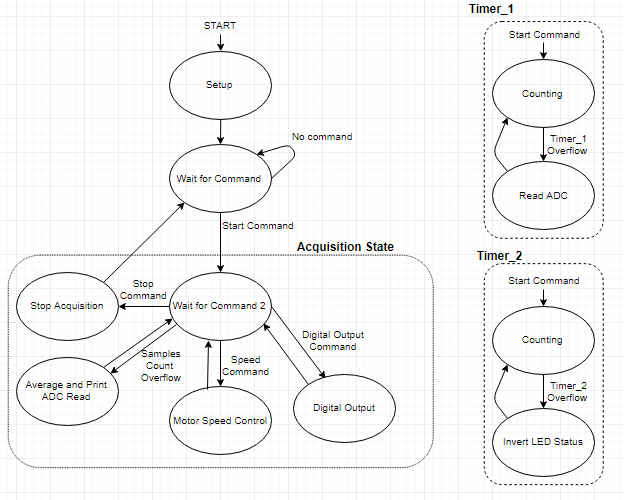
\includegraphics[scale=1]{figuras/fig-microCodeMap}
		\caption{Microcontroller Code Map \cite{microCodeMap}}
		\label{fig:microCode}
	\end{figure}
	
	
	As soon as the microcontroller is turned on it enters in the \textit{Setup}, on this part the following things are setted:
	\begin{itemize}
		\item \textit{Timer\_1: } Timer\_1 max count value is setted and a interruption service routine is appointed.\label{itm:mcu-prog-timer1}
		\item \textit{Timer\_2: } Same thing done for Timer\_1 is done for Timer\_2.\label{itm:mcu-prog-timer2}
		\item \textit{Serial Port: } The serial port baud rate is defined and the serial port is opened.\label{itm:mcu-prog-serial-port}
		\item \textit{Port definitions: } The I/O ports are defined as inputs (high impedance) or as outputs (low impedance).\label{itm:mcu-prog-port}
	\end{itemize}
	
	After setting up the code enters in a state in which it waits for a \textit{Start Command} from the computer. This command starts Timer\_1 and makes the code enter the \textit{Acquisition State}. Everytime Timer\_1 finishes its count a ISR will be triggered, all the analog inputs will be read (sampled) and stored followed by the timer restarting its counting process. The \textit{Start Command} also starts Timer\_2, this timer operates the same way as Timer\_1, the difference is that its ISR will only toggle the acquistion LED state.
	\par
	In the acquistion state, if a \textit{Digital Output Command} is received the code will decrypt this command (this is actually a group of possible commands) and set the digital outputs according to the decrypted message.
	\par
	A received \textit{Speed Command} instruction will make the code behave in a similar way than \textit{Digital Output Command}, code will decript the command (it also is a group of possible commands) and output a corresponding PWM value in the analog output port in order to control the electric motor speed.
	\par
	During all the \textit{Acquisition State}, everytime Timer\_1 ISR does a presetted number of reads, the code makes an average of thoose reads and will send them through the serial port to the computer. After that the code will reset the number of read samples and start to count samples again. Another useful feature is that during all the \textit{Acquisition State} the code is also continuosly reading the microcontroller digital inputs, this inputs are used to detect if a sensor is not connected, if any of the sensors is considered to be disconnected instead of sending the analog reading from the respective sensor input, the code will send a ``-1'' value to the computer. This way the computer software that the one responsible for treating this event and take the appropriate action.
	\par
	The code will exit the \textit{Acquisition State} if the computer sends a \textit{Stop Command}. This will also set all digital outputs to a low logic level and will disable both timers interruption service routines. The code will go back to the \textit{Wait for Command} state and wait for a \textit{Start Command} to restart acquisition. 
	\par
	This code architecture was designed in order to make the microcontroller code as simples as possible in order to make execution faster to avoid jeopardizing the real-time constrain. The same code is used during brake tests, during acquisition and any other process. As mentioned before, all the heavy data processing is done by the computer software.